\documentclass[11pt,a4paper]{article}

\usepackage[T1]{fontenc}
\usepackage[utf8]{inputenc}
\usepackage[spanish]{babel}
\usepackage{amsmath,amssymb}
\usepackage{graphicx}
\usepackage{booktabs}
\usepackage{geometry}
\usepackage{xcolor}
\usepackage{hyperref}
\geometry{margin=2.25cm}
\hypersetup{colorlinks=true, linkcolor=blue, urlcolor=blue, citecolor=blue}

% Generated by make_report_figures.py; do not edit manually.
\newcommand{\MaxDfourStressError}{1.963\times 10^{-6}}
\newcommand{\MaxDfourStrainError}{2.150\times 10^{-6}}
\newcommand{\MaxDfourEnergyError}{8.820\times 10^{-7}}
\newcommand{\MaxIsoStressMismatch}{1.556\times 10^{-2}}
\newcommand{\MaxIsoEnergyMismatch}{3.714\times 10^{-3}}
\newcommand{\IsoStressA}{8.762\times 10^{-3}}
\newcommand{\IsoEnergyA}{3.714\times 10^{-3}}
\newcommand{\IsoStressB}{1.556\times 10^{-2}}
\newcommand{\IsoEnergyB}{3.217\times 10^{-3}}
\newcommand{\IsoStressC}{2.786\times 10^{-3}}
\newcommand{\IsoEnergyC}{1.051\times 10^{-3}}


\newcommand{\Dfour}{\ensuremath{D_4}}
\newcommand{\Sbar}{\ensuremath{\overline{\mathbf S}}}
\newcommand{\Psibar}{\ensuremath{\overline{\Psi}}}

\title{Verificación FOM de la simetría efectiva del RVE\\
\large Por qué la PANN debe respetar \Dfour\ y no isotropía completa}
\author{Experimento reproducible con Kratos Eigen}
\date{\today}

\begin{document}
\maketitle

\begin{abstract}
Este documento explica el primer experimento físico que guía el diseño de la
PANN: identificar la simetría material efectiva del RVE hiperelástico con un
hueco circular central. Se ejecutaron casos FOM con Kratos Eigen para estados
de deformación transformados por las operaciones del cuadrado. El resultado es
inequívoco: las igualdades de \Dfour\ se cumplen a error numérico del orden de
$10^{-6}$, mientras que una rotación material de $45^\circ$ produce diferencias
de hasta \(\MaxIsoStressMismatch\) en tensión. El RVE representado por esta
geometría, malla y condiciones de contorno tiene simetría cuadrada \Dfour, no
isotropía completa.
\end{abstract}

\section{Pregunta física}

Antes de elegir invariantes o arquitecturas de red, hay que responder una
pregunta física: \emph{si aplicamos la misma deformación relativa al material,
pero girada respecto de los ejes del RVE, la energía efectiva es la misma?}
La respuesta determina qué simetría debe imponer la PANN.

El RVE considerado es un cuadrado con hueco circular centrado, material
Neo-Hookeano isotrópico y desplazamiento afín impuesto sobre la frontera
exterior. El material constituyente es isotrópico localmente, pero la celda
finita tiene la geometría mostrada en la Figura~\ref{fig:rve}: sólo conserva
rotaciones de $90^\circ$ y reflexiones, no cualquier ángulo.

\begin{figure}[ht]
  \centering
  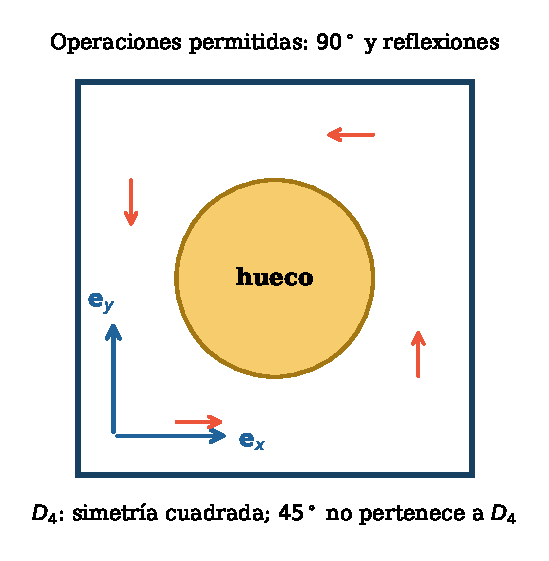
\includegraphics[width=0.66\linewidth]{figures/rve_square_symmetry_schematic.pdf}
  \caption{Geometría idealizada del RVE y sus operaciones de simetría material.
  Una rotación de $45^\circ$ no transforma el cuadrado en sí mismo.}
  \label{fig:rve}
\end{figure}

\section{Qué entra al solver y por qué la prueba usa deformación}

La base de datos y el solver usan como entrada la deformación de
Green--Lagrange en convención de Voigt,
\begin{equation}
 \mathbf e = [E_{11},E_{22},\gamma_{12}]^T,
 \qquad \gamma_{12}=2E_{12},
 \qquad
 \mathbf E=
 \begin{bmatrix}
 E_{11} & \gamma_{12}/2\\
 \gamma_{12}/2 & E_{22}
 \end{bmatrix}.
\end{equation}
El solver reconstruye internamente
\begin{equation}
 \mathbf C = \mathbf I+2\mathbf E,
 \qquad
 \mathbf F=\mathbf U=\mathbf C^{1/2},
\end{equation}
de modo que sólo se admiten estados con $\mathbf C$ definida positiva. Por
tanto, no es necesario cambiar la interfaz del solver a $\mathbf F$ para
verificar simetría material.

Para una rotación o reflexión material $\mathbf R$, la prueba se formula
directamente como
\begin{equation}
 \mathbf E' = \mathbf R^T\mathbf E\mathbf R,
 \qquad
 \mathbf C'=\mathbf R^T\mathbf C\mathbf R.
 \label{eq:input-transform}
\end{equation}
Por ejemplo,
\begin{align}
 [E_{11},E_{22},\gamma_{12}]^T
 &\xrightarrow{\text{reflexión }x}
 [E_{11},E_{22},-\gamma_{12}]^T,\\
 [E_{11},E_{22},\gamma_{12}]^T
 &\xrightarrow{90^\circ}
 [E_{22},E_{11},-\gamma_{12}]^T.
\end{align}

Esta \textbf{no} es una prueba de objetividad. La objetividad compara
$\mathbf F$ con $\mathbf Q\mathbf F$ al cambiar el observador espacial. Aquí
se cambia la orientación de la carga respecto de los ejes materiales del RVE,
lo cual comprueba su \textbf{simetría material}.

\section{Hipótesis que se comprueba}

La simetría cuadrada efectiva afirma que, para todo $\mathbf R\in\Dfour$,
\begin{equation}
 \Psibar(\mathbf R^T\mathbf C\mathbf R)=\Psibar(\mathbf C),
 \qquad
 \Sbar(\mathbf R^T\mathbf C\mathbf R)
 =\mathbf R^T\Sbar(\mathbf C)\mathbf R.
 \label{eq:d4}
\end{equation}
El grupo \Dfour\ tiene ocho matrices, pero $\mathbf R$ y $-\mathbf R$ tienen
la misma acción sobre el tensor simétrico $\mathbf E$. Por ello se probaron las
cuatro acciones distintas: identidad, reflexión respecto a $x$, rotación de
$90^\circ$ y reflexión diagonal.

Se usaron tres estados combinados, con extensión, compresión y cizalla:
\begin{center}
\begin{tabular}{c|rrr}
\toprule
Estado & $E_{11}$ & $E_{22}$ & $\gamma_{12}$\\
\midrule
A & 0.12 & -0.04 & 0.10\\
B & -0.06 & 0.09 & -0.12\\
C & 0.05 & 0.14 & 0.18\\
\bottomrule
\end{tabular}
\end{center}

La salida de tensión almacenada por el FOM es
$[S_{11},S_{22},S_{12}]^T$. Para cuantificar la igualdad de la
Ecuación~\eqref{eq:d4}, se evaluó
\begin{equation}
 e_S(\mathbf R)=
 \frac{\left\|\Sbar(\mathbf R^T\mathbf C\mathbf R)
 -\mathbf R^T\Sbar(\mathbf C)\mathbf R\right\|_2}
 {\max\left(\left\|\mathbf R^T\Sbar(\mathbf C)\mathbf R\right\|_2,10^{-14}\right)}.
\end{equation}

La energía no se dedujo de una curva dibujada. Se evaluó directamente en los
puntos de Gauss convergidos mediante
\begin{equation}
 \Psibar \approx \frac{1}{A_0}\sum_e A_e\frac{1}{n_g}
 \sum_{g=1}^{n_g}\psi(\mathbf C_{eg}),
\end{equation}
donde, para el Neo-Hookeano compresible en deformación plana,
\begin{equation}
 \psi = \frac{\mu}{2}\left(\mathrm{tr}\,\mathbf C-2\right)
       -\mu\ln J + \frac{\lambda}{2}(\ln J)^2,
 \qquad J=\sqrt{\det\mathbf C}.
\end{equation}

\section{Resultado: la simetría \Dfour\ se cumple}

La Figura~\ref{fig:d4errors} muestra los errores para todas las transformaciones
no triviales. Los máximos globales son
\begin{equation}
 \max e_S=\MaxDfourStressError,
 \qquad
 \max e_{\overline{\mathbf E}}=\MaxDfourStrainError,
 \qquad
 \max e_{\Psi}=\MaxDfourEnergyError.
\end{equation}
Estos valores son compatibles con la tolerancia Newton y con la pequeña falta
de simetría nodo-a-nodo de una malla no estructurada. No son una discrepancia
material apreciable.

\begin{figure}[ht]
  \centering
  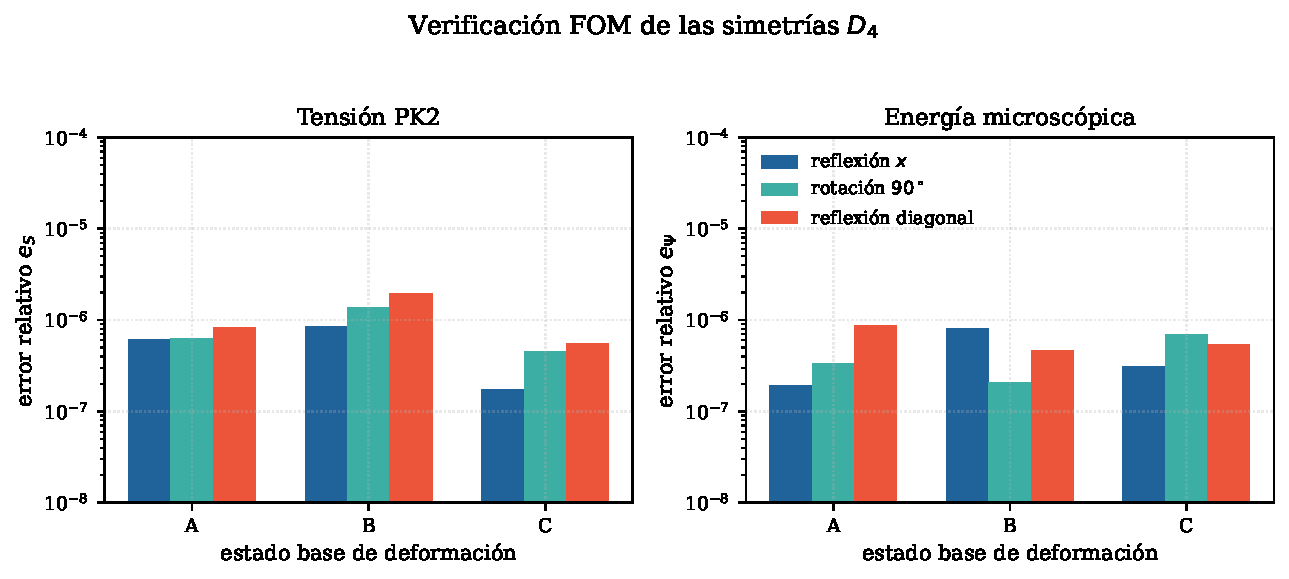
\includegraphics[width=\linewidth]{figures/d4_symmetry_errors.pdf}
  \caption{Errores relativos de tensión y energía bajo las operaciones de
  simetría cuadrada. La escala logarítmica muestra que todos están en torno a
  $10^{-6}$ o menos.}
  \label{fig:d4errors}
\end{figure}

\section{Control negativo: una rotación de $45^\circ$}

La igualdad isotrópica exigiría la Ecuación~\eqref{eq:d4} para \emph{cualquier}
rotación $\mathbf R\in SO(2)$, incluyendo
\begin{equation}
 \mathbf R_{45}=
 \begin{bmatrix}
 1/\sqrt{2} & -1/\sqrt{2}\\
 1/\sqrt{2} &  1/\sqrt{2}
 \end{bmatrix}.
\end{equation}
Sin embargo, $\mathbf R_{45}\notin\Dfour$. El contraste numérico de la
Figura~\ref{fig:isotropy} da discrepancias entre $0.278\%$ y $1.556\%$ en
tensión, y entre $0.105\%$ y $0.371\%$ en energía. Estas diferencias son entre
aproximadamente mil y diez mil veces mayores que los errores de \Dfour.

\begin{figure}[ht]
  \centering
  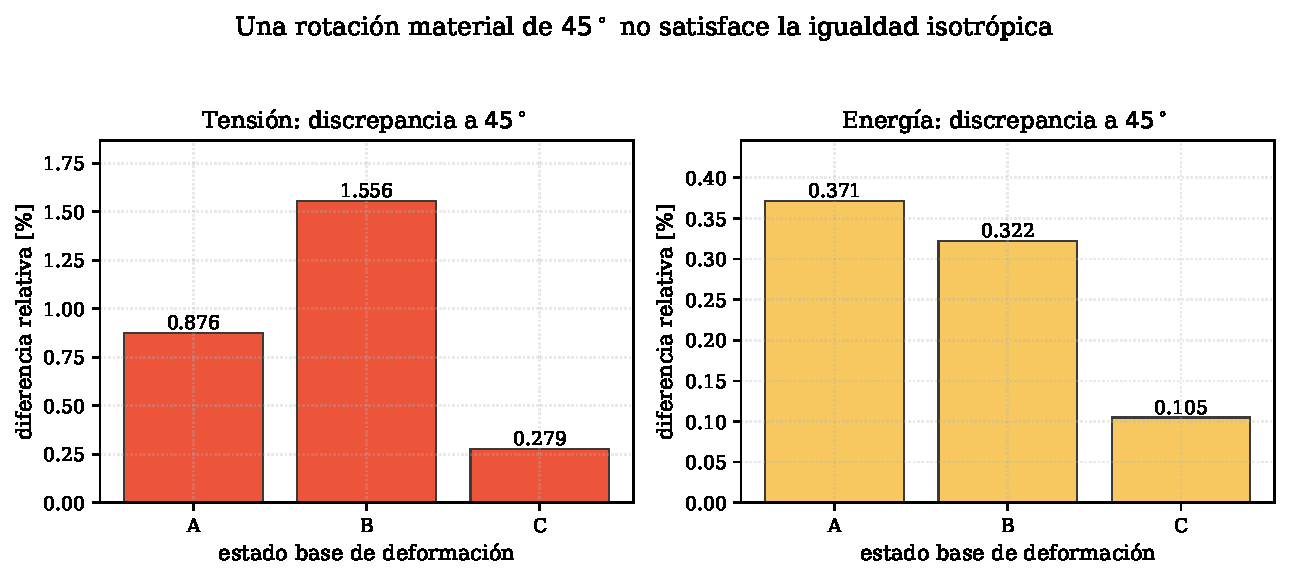
\includegraphics[width=\linewidth]{figures/isotropy_45_degree_mismatch.pdf}
  \caption{Discrepancia del FOM frente a la respuesta que predeciría una ley
  isotrópica bajo una rotación material de $45^\circ$. Las diferencias son
  físicas, no ruido numérico.}
  \label{fig:isotropy}
\end{figure}

\section{Conclusión para la PANN}

La conclusión de este experimento es
\begin{equation}
 \boxed{\text{El RVE efectivo es \Dfour\text{-simétrico, no isótropo.}}}
\end{equation}
Por ello, una PANN basada sólo en deformaciones principales impondría más
simetría de la que tiene el problema. La construcción recomendada es una
energía objetiva basada en $\mathbf C$ y simetrizada exactamente sobre \Dfour,
\begin{equation}
 \widetilde\Psi_\theta(\mathbf C)=
 \frac{1}{8}\sum_{\mathbf R\in\Dfour}
 \Psi_{\mathrm{base},\theta}(\mathbf R^T\mathbf C\mathbf R),
 \qquad
 \Sbar_\theta=2\frac{\partial\widetilde\Psi_\theta}{\partial\mathbf C}.
\end{equation}
Después se impondrá el estado de referencia
$\widetilde\Psi_\theta(\mathbf I)=0$ y
$\Sbar_\theta(\mathbf I)=\mathbf 0$. ICNN e ICKAN pueden actuar como
$\Psi_{\mathrm{base},\theta}$, pero la simetrización \Dfour\ debe ser común a
ambas arquitecturas.

\paragraph{Alcance honesto.} Esta prueba identifica la simetría de la
geometría, malla y condiciones de contorno actualmente usadas. Para el artículo
final habrá que repetirla en más estados de deformación y, preferiblemente, en
una malla refinada. No demuestra por sí sola estabilidad global, policonvexidad
ni generalización de una PANN; sí fija de manera cuantitativa la simetría que
la PANN debe respetar.

\end{document}
